\documentclass[twoside]{book}

% Packages required by doxygen
\usepackage{fixltx2e}
\usepackage{calc}
\usepackage{doxygen}
\usepackage[export]{adjustbox} % also loads graphicx
\usepackage{graphicx}
\usepackage[utf8]{inputenc}
\usepackage{makeidx}
\usepackage{multicol}
\usepackage{multirow}
\PassOptionsToPackage{warn}{textcomp}
\usepackage{textcomp}
\usepackage[nointegrals]{wasysym}
\usepackage[table]{xcolor}

% Font selection
\usepackage[T1]{fontenc}
\usepackage[scaled=.90]{helvet}
\usepackage{courier}
\usepackage{amssymb}
\usepackage{sectsty}
\renewcommand{\familydefault}{\sfdefault}
\allsectionsfont{%
  \fontseries{bc}\selectfont%
  \color{darkgray}%
}
\renewcommand{\DoxyLabelFont}{%
  \fontseries{bc}\selectfont%
  \color{darkgray}%
}
\newcommand{\+}{\discretionary{\mbox{\scriptsize$\hookleftarrow$}}{}{}}

% Page & text layout
\usepackage{geometry}
\geometry{%
  a4paper,%
  top=2.5cm,%
  bottom=2.5cm,%
  left=2.5cm,%
  right=2.5cm%
}
\tolerance=750
\hfuzz=15pt
\hbadness=750
\setlength{\emergencystretch}{15pt}
\setlength{\parindent}{0cm}
\setlength{\parskip}{3ex plus 2ex minus 2ex}
\makeatletter
\renewcommand{\paragraph}{%
  \@startsection{paragraph}{4}{0ex}{-1.0ex}{1.0ex}{%
    \normalfont\normalsize\bfseries\SS@parafont%
  }%
}
\renewcommand{\subparagraph}{%
  \@startsection{subparagraph}{5}{0ex}{-1.0ex}{1.0ex}{%
    \normalfont\normalsize\bfseries\SS@subparafont%
  }%
}
\makeatother

% Headers & footers
\usepackage{fancyhdr}
\pagestyle{fancyplain}
\fancyhead[LE]{\fancyplain{}{\bfseries\thepage}}
\fancyhead[CE]{\fancyplain{}{}}
\fancyhead[RE]{\fancyplain{}{\bfseries\leftmark}}
\fancyhead[LO]{\fancyplain{}{\bfseries\rightmark}}
\fancyhead[CO]{\fancyplain{}{}}
\fancyhead[RO]{\fancyplain{}{\bfseries\thepage}}
\fancyfoot[LE]{\fancyplain{}{}}
\fancyfoot[CE]{\fancyplain{}{}}
\fancyfoot[RE]{\fancyplain{}{\bfseries\scriptsize Generated by Doxygen }}
\fancyfoot[LO]{\fancyplain{}{\bfseries\scriptsize Generated by Doxygen }}
\fancyfoot[CO]{\fancyplain{}{}}
\fancyfoot[RO]{\fancyplain{}{}}
\renewcommand{\footrulewidth}{0.4pt}
\renewcommand{\chaptermark}[1]{%
  \markboth{#1}{}%
}
\renewcommand{\sectionmark}[1]{%
  \markright{\thesection\ #1}%
}

% Indices & bibliography
\usepackage{natbib}
\usepackage[titles]{tocloft}
\setcounter{tocdepth}{3}
\setcounter{secnumdepth}{5}
\makeindex

% Hyperlinks (required, but should be loaded last)
\usepackage{ifpdf}
\ifpdf
  \usepackage[pdftex,pagebackref=true]{hyperref}
\else
  \usepackage[ps2pdf,pagebackref=true]{hyperref}
\fi
\hypersetup{%
  colorlinks=true,%
  linkcolor=blue,%
  citecolor=blue,%
  unicode%
}

% Custom commands
\newcommand{\clearemptydoublepage}{%
  \newpage{\pagestyle{empty}\cleardoublepage}%
}

\usepackage{caption}
\captionsetup{labelsep=space,justification=centering,font={bf},singlelinecheck=off,skip=4pt,position=top}

%===== C O N T E N T S =====

\begin{document}

% Titlepage & ToC
\hypersetup{pageanchor=false,
             bookmarksnumbered=true,
             pdfencoding=unicode
            }
\pagenumbering{roman}
\begin{titlepage}
\vspace*{7cm}
\begin{center}%
{\Large My Project }\\
\vspace*{1cm}
{\large Generated by Doxygen 1.8.11}\\
\end{center}
\end{titlepage}
\clearemptydoublepage
\tableofcontents
\clearemptydoublepage
\pagenumbering{arabic}
\hypersetup{pageanchor=true}

%--- Begin generated contents ---
\chapter{Research Track I -\/ Final Assignment}
\label{md_README}
\hypertarget{md_README}{}
In this repository you will find a package required for the construction of an interface whose the scope is to take commands from the user and execute them. The possible commands are\+: 1) Reach a random target 2) Choose a target among some possibilities which are (-\/4,-\/3);(-\/4,2);(-\/4,7);(5,-\/7);(5,-\/3);(5,1) 3) Follow the wall 4) Stop the robot

\subsection*{Prerequisites}

To execute successfully the code, there are required two other package. Clone the following repository in you workspace\+:
\begin{DoxyItemize}
\item \href{https://github.com/CarmineD8/slam_gmapping}{\tt https\+://github.\+com/\+Carmine\+D8/slam\+\_\+gmapping}
\item \href{https://github.com/CarmineD8/final_assignment}{\tt https\+://github.\+com/\+Carmine\+D8/final\+\_\+assignment}
\end{DoxyItemize}

After the clonation of each package, do a catkin\+\_\+make.

\subsection*{Nodes}

\subsubsection*{\hyperlink{interface_8py}{interface.\+py}}

It takes the commands from the user and execute them

\subsubsection*{random\+\_\+service}

It generate the random target required for the first command

\subsection*{How the node communicate to each other}

You can find in the doc directory, the ros\+\_\+graph -\/$>$ it shows how the node communicate to each othere

\subsection*{How to run the code\+:}


\begin{DoxyItemize}
\item As first step it is necessary to run a command to create the master 
\begin{DoxyCode}
1 roscore & 
\end{DoxyCode}

\item As second step run the simulation space with 
\begin{DoxyCode}
1 roslaunch final\_assignment simulation\_gmapping.launch
\end{DoxyCode}

\item As third step in another shell use the command to run the launch move\+\_\+base 
\begin{DoxyCode}
1 roslaunch final\_assignment move\_base.launch
\end{DoxyCode}

\item As last step, in another shell, use the command to run the interface 
\begin{DoxyCode}
1 roslaunch triglia\_final\_assignment assignment2.launch
\end{DoxyCode}
 
\end{DoxyItemize}
\chapter{Namespace Index}
\section{Namespace List}
Here is a list of all namespaces with brief descriptions\+:\begin{DoxyCompactList}
\item\contentsline{section}{\hyperlink{namespaceinterface}{interface} }{\pageref{namespaceinterface}}{}
\end{DoxyCompactList}

\chapter{File Index}
\section{File List}
Here is a list of all files with brief descriptions\+:\begin{DoxyCompactList}
\item\contentsline{section}{scripts/\hyperlink{interface_8py}{interface.\+py} }{\pageref{interface_8py}}{}
\item\contentsline{section}{src/\hyperlink{random__service_8cpp}{random\+\_\+service.\+cpp} }{\pageref{random__service_8cpp}}{}
\end{DoxyCompactList}

\chapter{Namespace Documentation}
\hypertarget{namespaceinterface}{}\section{interface Namespace Reference}
\label{namespaceinterface}\index{interface@{interface}}
\subsection*{Functions}
\begin{DoxyCompactItemize}
\item 
def \hyperlink{namespaceinterface_a4dd15fe19a2580f21d8db65f681e01d0}{actual\+\_\+position} (odom\+\_\+data)
\item 
def \hyperlink{namespaceinterface_afb9c8042f33be80f7d047c827902cf6f}{move\+\_\+randomly\+\_\+to\+\_\+target} (target\+\_\+x, target\+\_\+y)
\begin{DoxyCompactList}\small\item\em The scope of move\+\_\+target is to use move\+\_\+base service to reach the target itself. \end{DoxyCompactList}\item 
def \hyperlink{namespaceinterface_a5307e508f28944b1b1b67cd5e9d16d60}{reaching\+\_\+the\+\_\+target} (target\+\_\+x, target\+\_\+y)
\item 
def \hyperlink{namespaceinterface_ae795c613b93f173e3b867be138002990}{user\+\_\+set\+\_\+position} ()
\item 
def \hyperlink{namespaceinterface_ac84656acec70183a4ef276f4a3343971}{main} ()
\end{DoxyCompactItemize}
\subsection*{Variables}
\begin{DoxyCompactItemize}
\item 
\hyperlink{namespaceinterface_a7e2f9384bca70d8ebd012646492277b3}{actual\+\_\+position} = Point()
\item 
\hyperlink{namespaceinterface_a1de259b3c06e4f436bbade32c75c9318}{pub\+\_\+goal} = None
\begin{DoxyCompactList}\small\item\em To publish new goals. \end{DoxyCompactList}\item 
\hyperlink{namespaceinterface_ac9f12ff0de8248506bf532b6874750e7}{sub\+\_\+odom} = None
\begin{DoxyCompactList}\small\item\em Initiliaze the wall\+\_\+follower client. \end{DoxyCompactList}\item 
\hyperlink{namespaceinterface_a4709d1a9f45323d007767a3b7c4725f5}{pub\+\_\+target\+\_\+reached} = None
\end{DoxyCompactItemize}


\subsection{Function Documentation}
\index{interface@{interface}!actual\+\_\+position@{actual\+\_\+position}}
\index{actual\+\_\+position@{actual\+\_\+position}!interface@{interface}}
\subsubsection[{\texorpdfstring{actual\+\_\+position(odom\+\_\+data)}{actual_position(odom_data)}}]{\setlength{\rightskip}{0pt plus 5cm}def interface.\+actual\+\_\+position (
\begin{DoxyParamCaption}
\item[{}]{odom\+\_\+data}
\end{DoxyParamCaption}
)}\hypertarget{namespaceinterface_a4dd15fe19a2580f21d8db65f681e01d0}{}\label{namespaceinterface_a4dd15fe19a2580f21d8db65f681e01d0}


Definition at line 23 of file interface.\+py.

\index{interface@{interface}!main@{main}}
\index{main@{main}!interface@{interface}}
\subsubsection[{\texorpdfstring{main()}{main()}}]{\setlength{\rightskip}{0pt plus 5cm}def interface.\+main (
\begin{DoxyParamCaption}
{}
\end{DoxyParamCaption}
)}\hypertarget{namespaceinterface_ac84656acec70183a4ef276f4a3343971}{}\label{namespaceinterface_ac84656acec70183a4ef276f4a3343971}


Definition at line 78 of file interface.\+py.

\index{interface@{interface}!move\+\_\+randomly\+\_\+to\+\_\+target@{move\+\_\+randomly\+\_\+to\+\_\+target}}
\index{move\+\_\+randomly\+\_\+to\+\_\+target@{move\+\_\+randomly\+\_\+to\+\_\+target}!interface@{interface}}
\subsubsection[{\texorpdfstring{move\+\_\+randomly\+\_\+to\+\_\+target(target\+\_\+x, target\+\_\+y)}{move_randomly_to_target(target_x, target_y)}}]{\setlength{\rightskip}{0pt plus 5cm}def interface.\+move\+\_\+randomly\+\_\+to\+\_\+target (
\begin{DoxyParamCaption}
\item[{}]{target\+\_\+x, }
\item[{}]{target\+\_\+y}
\end{DoxyParamCaption}
)}\hypertarget{namespaceinterface_afb9c8042f33be80f7d047c827902cf6f}{}\label{namespaceinterface_afb9c8042f33be80f7d047c827902cf6f}


The scope of move\+\_\+target is to use move\+\_\+base service to reach the target itself. 



Definition at line 28 of file interface.\+py.

\index{interface@{interface}!reaching\+\_\+the\+\_\+target@{reaching\+\_\+the\+\_\+target}}
\index{reaching\+\_\+the\+\_\+target@{reaching\+\_\+the\+\_\+target}!interface@{interface}}
\subsubsection[{\texorpdfstring{reaching\+\_\+the\+\_\+target(target\+\_\+x, target\+\_\+y)}{reaching_the_target(target_x, target_y)}}]{\setlength{\rightskip}{0pt plus 5cm}def interface.\+reaching\+\_\+the\+\_\+target (
\begin{DoxyParamCaption}
\item[{}]{target\+\_\+x, }
\item[{}]{target\+\_\+y}
\end{DoxyParamCaption}
)}\hypertarget{namespaceinterface_a5307e508f28944b1b1b67cd5e9d16d60}{}\label{namespaceinterface_a5307e508f28944b1b1b67cd5e9d16d60}


Definition at line 43 of file interface.\+py.

\index{interface@{interface}!user\+\_\+set\+\_\+position@{user\+\_\+set\+\_\+position}}
\index{user\+\_\+set\+\_\+position@{user\+\_\+set\+\_\+position}!interface@{interface}}
\subsubsection[{\texorpdfstring{user\+\_\+set\+\_\+position()}{user_set_position()}}]{\setlength{\rightskip}{0pt plus 5cm}def interface.\+user\+\_\+set\+\_\+position (
\begin{DoxyParamCaption}
{}
\end{DoxyParamCaption}
)}\hypertarget{namespaceinterface_ae795c613b93f173e3b867be138002990}{}\label{namespaceinterface_ae795c613b93f173e3b867be138002990}


Definition at line 60 of file interface.\+py.



\subsection{Variable Documentation}
\index{interface@{interface}!actual\+\_\+position@{actual\+\_\+position}}
\index{actual\+\_\+position@{actual\+\_\+position}!interface@{interface}}
\subsubsection[{\texorpdfstring{actual\+\_\+position}{actual_position}}]{\setlength{\rightskip}{0pt plus 5cm}interface.\+actual\+\_\+position = Point()}\hypertarget{namespaceinterface_a7e2f9384bca70d8ebd012646492277b3}{}\label{namespaceinterface_a7e2f9384bca70d8ebd012646492277b3}


Definition at line 13 of file interface.\+py.

\index{interface@{interface}!pub\+\_\+goal@{pub\+\_\+goal}}
\index{pub\+\_\+goal@{pub\+\_\+goal}!interface@{interface}}
\subsubsection[{\texorpdfstring{pub\+\_\+goal}{pub_goal}}]{\setlength{\rightskip}{0pt plus 5cm}interface.\+pub\+\_\+goal = None}\hypertarget{namespaceinterface_a1de259b3c06e4f436bbade32c75c9318}{}\label{namespaceinterface_a1de259b3c06e4f436bbade32c75c9318}


To publish new goals. 



Definition at line 16 of file interface.\+py.

\index{interface@{interface}!pub\+\_\+target\+\_\+reached@{pub\+\_\+target\+\_\+reached}}
\index{pub\+\_\+target\+\_\+reached@{pub\+\_\+target\+\_\+reached}!interface@{interface}}
\subsubsection[{\texorpdfstring{pub\+\_\+target\+\_\+reached}{pub_target_reached}}]{\setlength{\rightskip}{0pt plus 5cm}interface.\+pub\+\_\+target\+\_\+reached = None}\hypertarget{namespaceinterface_a4709d1a9f45323d007767a3b7c4725f5}{}\label{namespaceinterface_a4709d1a9f45323d007767a3b7c4725f5}


Definition at line 21 of file interface.\+py.

\index{interface@{interface}!sub\+\_\+odom@{sub\+\_\+odom}}
\index{sub\+\_\+odom@{sub\+\_\+odom}!interface@{interface}}
\subsubsection[{\texorpdfstring{sub\+\_\+odom}{sub_odom}}]{\setlength{\rightskip}{0pt plus 5cm}interface.\+sub\+\_\+odom = None}\hypertarget{namespaceinterface_ac9f12ff0de8248506bf532b6874750e7}{}\label{namespaceinterface_ac9f12ff0de8248506bf532b6874750e7}


Initiliaze the wall\+\_\+follower client. 



Definition at line 19 of file interface.\+py.


\chapter{File Documentation}
\hypertarget{_r_e_a_d_m_e_8md}{}\section{R\+E\+A\+D\+M\+E.\+md File Reference}
\label{_r_e_a_d_m_e_8md}\index{R\+E\+A\+D\+M\+E.\+md@{R\+E\+A\+D\+M\+E.\+md}}

\hypertarget{interface_8py}{}\section{scripts/interface.py File Reference}
\label{interface_8py}\index{scripts/interface.\+py@{scripts/interface.\+py}}
\subsection*{Namespaces}
\begin{DoxyCompactItemize}
\item 
 \hyperlink{namespaceinterface}{interface}
\end{DoxyCompactItemize}
\subsection*{Functions}
\begin{DoxyCompactItemize}
\item 
def \hyperlink{namespaceinterface_a4dd15fe19a2580f21d8db65f681e01d0}{interface.\+actual\+\_\+position} (odom\+\_\+data)
\item 
def \hyperlink{namespaceinterface_afb9c8042f33be80f7d047c827902cf6f}{interface.\+move\+\_\+randomly\+\_\+to\+\_\+target} (target\+\_\+x, target\+\_\+y)
\begin{DoxyCompactList}\small\item\em The scope of move\+\_\+target is to use move\+\_\+base service to reach the target itself. \end{DoxyCompactList}\item 
def \hyperlink{namespaceinterface_a5307e508f28944b1b1b67cd5e9d16d60}{interface.\+reaching\+\_\+the\+\_\+target} (target\+\_\+x, target\+\_\+y)
\item 
def \hyperlink{namespaceinterface_ae795c613b93f173e3b867be138002990}{interface.\+user\+\_\+set\+\_\+position} ()
\item 
def \hyperlink{namespaceinterface_ac84656acec70183a4ef276f4a3343971}{interface.\+main} ()
\end{DoxyCompactItemize}
\subsection*{Variables}
\begin{DoxyCompactItemize}
\item 
\hyperlink{namespaceinterface_a7e2f9384bca70d8ebd012646492277b3}{interface.\+actual\+\_\+position} = Point()
\item 
\hyperlink{namespaceinterface_a1de259b3c06e4f436bbade32c75c9318}{interface.\+pub\+\_\+goal} = None
\begin{DoxyCompactList}\small\item\em To publish new goals. \end{DoxyCompactList}\item 
\hyperlink{namespaceinterface_ac9f12ff0de8248506bf532b6874750e7}{interface.\+sub\+\_\+odom} = None
\begin{DoxyCompactList}\small\item\em Initiliaze the wall\+\_\+follower client. \end{DoxyCompactList}\item 
\hyperlink{namespaceinterface_a4709d1a9f45323d007767a3b7c4725f5}{interface.\+pub\+\_\+target\+\_\+reached} = None
\end{DoxyCompactItemize}

\hypertarget{random__service_8cpp}{}\section{src/random\+\_\+service.cpp File Reference}
\label{random__service_8cpp}\index{src/random\+\_\+service.\+cpp@{src/random\+\_\+service.\+cpp}}
{\ttfamily \#include \char`\"{}ros/ros.\+h\char`\"{}}\\*
{\ttfamily \#include \char`\"{}triglia\+\_\+final\+\_\+assignment/\+Server2.\+h\char`\"{}}\\*
{\ttfamily \#include $<$math.\+h$>$}\\*
Include dependency graph for random\+\_\+service.\+cpp\+:
\nopagebreak
\begin{figure}[H]
\begin{center}
\leavevmode
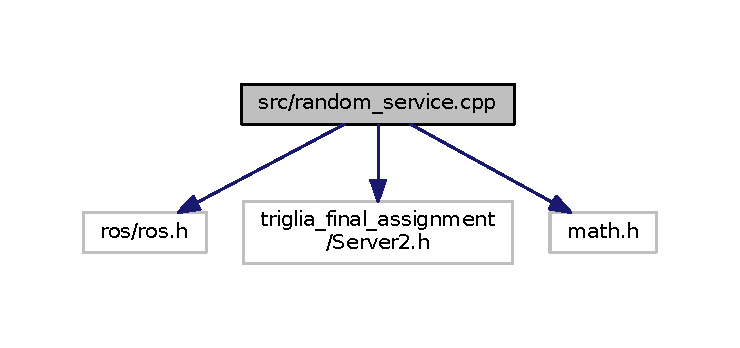
\includegraphics[width=350pt]{random__service_8cpp__incl}
\end{center}
\end{figure}
\subsection*{Functions}
\begin{DoxyCompactItemize}
\item 
bool \hyperlink{random__service_8cpp_a07928824e1d4a2dc2cdccfdd71c3410f}{pos\+\_\+random} (triglia\+\_\+final\+\_\+assignment\+::\+Server2\+::\+Request \&req, triglia\+\_\+final\+\_\+assignment\+::\+Server2\+::\+Response \&res)
\item 
int \hyperlink{random__service_8cpp_a3c04138a5bfe5d72780bb7e82a18e627}{main} (int argc, char $\ast$$\ast$argv)
\end{DoxyCompactItemize}


\subsection{Function Documentation}
\index{random\+\_\+service.\+cpp@{random\+\_\+service.\+cpp}!main@{main}}
\index{main@{main}!random\+\_\+service.\+cpp@{random\+\_\+service.\+cpp}}
\subsubsection[{\texorpdfstring{main(int argc, char $\ast$$\ast$argv)}{main(int argc, char **argv)}}]{\setlength{\rightskip}{0pt plus 5cm}int main (
\begin{DoxyParamCaption}
\item[{int}]{argc, }
\item[{char $\ast$$\ast$}]{argv}
\end{DoxyParamCaption}
)}\hypertarget{random__service_8cpp_a3c04138a5bfe5d72780bb7e82a18e627}{}\label{random__service_8cpp_a3c04138a5bfe5d72780bb7e82a18e627}


Definition at line 20 of file random\+\_\+service.\+cpp.

\index{random\+\_\+service.\+cpp@{random\+\_\+service.\+cpp}!pos\+\_\+random@{pos\+\_\+random}}
\index{pos\+\_\+random@{pos\+\_\+random}!random\+\_\+service.\+cpp@{random\+\_\+service.\+cpp}}
\subsubsection[{\texorpdfstring{pos\+\_\+random(triglia\+\_\+final\+\_\+assignment\+::\+Server2\+::\+Request \&req, triglia\+\_\+final\+\_\+assignment\+::\+Server2\+::\+Response \&res)}{pos_random(triglia_final_assignment::Server2::Request &req, triglia_final_assignment::Server2::Response &res)}}]{\setlength{\rightskip}{0pt plus 5cm}bool pos\+\_\+random (
\begin{DoxyParamCaption}
\item[{triglia\+\_\+final\+\_\+assignment\+::\+Server2\+::\+Request \&}]{req, }
\item[{triglia\+\_\+final\+\_\+assignment\+::\+Server2\+::\+Response \&}]{res}
\end{DoxyParamCaption}
)}\hypertarget{random__service_8cpp_a07928824e1d4a2dc2cdccfdd71c3410f}{}\label{random__service_8cpp_a07928824e1d4a2dc2cdccfdd71c3410f}


Definition at line 7 of file random\+\_\+service.\+cpp.


%--- End generated contents ---

% Index
\backmatter
\newpage
\phantomsection
\clearemptydoublepage
\addcontentsline{toc}{chapter}{Index}
\printindex

\end{document}
